\subsection*{Information and Signals}
\textbf{Nomenclature:}

\underline{Signal power}: $S$ [W]

\underline{Bandwidth}: $B$ [Hz]

\underline{Noise power}: $N$ [W]

\underline{Bit energy}: $E_b$ [J]

\underline{Noise spectral density}: $N_0=-174[\text{dBm}]$ [W/Hz]

\underline{Transmission channel capacity}: $C$ [bits/s]

\underline{Transmission speed}: $R$ [bits/s]

\underline{Total number of distinct modulation states}: $M$

\underline{La dégradation due au récepteur}: $NF$

\textbf{Signal:}

\underline{AWGN} (additive white Gaussian noise) est un modèle de bruit.
\begin{figure}[H]
    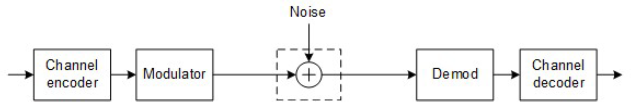
\includegraphics[width=\linewidth]{images/awgn_channel_model.png}
\end{figure}
\underline{Puissance en dBm}: $P_{dBm} = 10\log_{10}\left(\frac{P}{1mW}\right)$

\underline{Noise power}: $N = N_0B$

\underline{Channel capacity}: $C = B\log_2\left(1+\frac{S}{N}\right)$

\underline{Signal power}: $S = E_bR$

\underline{Rendement}: $\frac{E_b}{N_0}=\frac{2^{\sfrac{C}{B}}-1}{\sfrac{R}{B}}$

\underline{BER}: $\frac{1}{2}\cdot\text{erfc}\left(\sqrt{\frac{E_b}{N_0}}\right)$

\textbf{Information:}

L'alphabet numérique est fait de 0 et 1 avec des probabilités
égales $P(0) = P(1)$. Le niveau zéro (0V) est inadapté pour le symbole 0. On attribue
donc 1 au symbole 1 et -1 au symbole 0.

Bit d'information peut être un symbol électrique de forme variable.
Un signal Gaussien est un symbol idéal, c'est une Gaussienne en temps et fréquence.
Plus la Gausienne est étroite en temps, plus le signal est large en fréquence et
vice-versa. L'espacement des symboles est limité par la durée de l'impulsion et
donc par la bande passante $B$

\underline{Nombre de symbols par unité de temps:} $R_b \leq 2B[\sfrac{\text{symbol}}{s}\text{ ou bauds}]$

L'interférence Inter Symbol (ISI) est causée par le dépassement de cette limite.

Un signal numérique doit être filtré passe-bas pour limiter sa bande passante.
Un canal fréquentiel optimal serait un $rect()$, dont la transformée de Fourier inverse
est un $sinc()$. Le pulse en $sinc()$ est théoriquement optimal, mais pratiquement

\setlength{\abovedisplayskip}{-5pt}
\setlength{\belowdisplayskip}{-5pt}
\begin{wrapfigure}{l}{11cm}
    \begin{equation*}
        P(f)=\begin{cases}
            T_S                                                                                                       & \text{si } 0<|f| < \frac{1-\alpha}{2T_S}                       \\
            \frac{T_S}{2}\left[1+\cos\left(\frac{\pi T_S}{\alpha}\left(|f|-\frac{1-\alpha}{2T_S}\right)\right)\right] & \text{si } \frac{1-\alpha}{2T_S} < |f| < \frac{1+\alpha}{2T_S} \\
            0                                                                                                         & \text{sinon}
        \end{cases}
    \end{equation*}
\end{wrapfigure}
inviable, car il nécessite un filtre d'ordre très élevé et il est sensible aux erreurs
temporelles qui créent de l'ISI.
On préfère donc utiliser un \underline{quadrant de sinus (raised cosine)}: $p(t) = \frac{\sin(\sfrac{\pi t}{T_S})}{\sfrac{\pi t}{T_S}}\cdot\frac{\cos(\sfrac{\alpha\pi t}{T_S})}{1-(\sfrac{\alpha t}{T_S})^2}$

Le roll-off factor $\alpha$ permet de contrôler la bande passante du signal.

\underline{Débit binaire}: $R_b = \frac{2B}{1+\alpha}$.

On souhaite filtrer à l'émission pour respecter le canal RF mais aussi à la réception
pour retrouver le signal d'origine après passage dans le canal. Une solution est de
séparer le filtre RC en deux par deux filtres RRC (Root Raised Cosine) un à l'émission et
un à la réception.

\underline{Priorité du filtre RRC}: $\left|H_{rc}(f)\right|=\sqrt{\left|H_{rrc}(f)\right|}\cdot\sqrt{\left|H_{rrc}(f)\right|}=\left|H_{rrc}(f)\right|\cdot \left|H_{rrc}(f)\right|$.